\documentclass[iop]{emulateapj-rtx4}
%\documentclass[twocolumn,tighten]{aastex6}
%\documentclass{aastex6}
%\usepackage{emulateapj-rtx4}
%\usepackage{emulateapj}

 \shortauthors{French $\&$ Wakker}

\usepackage{graphicx}
\usepackage{subfigure}
%\usepackage{amssymb}
%\usepackage{wrapfig}
%\usepackage{setspace}

%\usepackage{mathtools}
%\frenchspacing
\graphicspath{{figures//}}

\begin{document}

\title{Ly$\alpha$ absorbers do/not co-rotate with galaxy disks}

\author{David M. French, Bart P. Wakker}

\affil{Department of Astronomy, University of Wisconsin, Madison, WI 53706, USA}

\begin{abstract}

We present results of a study comparing the relative velocity of Ly$\alpha$ absorbers to the rotation direction and velocity of nearby galaxy disks. We find...

\end{abstract}


\keywords{galaxies:intergalactic medium, galaxies:evolution, galaxies:halos, quasars: absorption lines}


\section{INTRODUCTION}



\begin{table*}[ht]\footnotesize
\begin{center}
\begin{tabular}{l l l l l l l l l l}
 \hline \hline
  Target 		& R.A. 		& Dec. 		& \textit{z}		 & Program 	  & Grating 	  & Obs ID 	    & Obs Date 	    & $T_{exp}*$     & S/N*  \\ 
  	    		& 	       		&	  		& 		  	 & 		    	  & 		  	  & 		  	   & 		     	    & 	        [ks]        & [1238] \\ 
 \scriptsize (1)  & \scriptsize (2) & \scriptsize (3) & \scriptsize (4) & \scriptsize (5) & \scriptsize (6) & \scriptsize  (7) & \scriptsize (8) & \scriptsize (9) & \scriptsize (10)  \\ \hline \hline
\\
    
1H0717+714		  &  7.0  21.0   53.3  &     71.0  20.0  36.0  &    0.5003  & 12025  	    &   G130M  &   LBG812  		 & 11-12-27      	 	  &  6.0    &      37         \\

 \\
\hline

\end{tabular}
\end{center}
  \caption{\small{COS targets in this sample. *Total exposure time and S/N ratio is given for multi-orbit exposures.}}
  \label{target_table}
\end{table*}


\section{DATA AND ANALYSIS}

\subsection{SALT Data}



\subsection{Ancillary Data}


\subsection{Galaxy Data}


%\begin{figure}[ht!]
%        \centering
%        \vspace{0pt}
%        \includegraphics[width=0.50\textwidth]{fig1.pdf}
%        \caption{\small{Distribution of $L/L_{\**}$ values for all galaxies in the dataset. Black vertical lines highlight 1, 0.5, 0.1, 0.05 and 0.01 $L_{\**}$. The turnoff around 0.1$L_{\**}$ shows that on average, the dataset is mostly complete to 0.2$L_{\**}$.}}
%%        \vspace{-5pt}
%        \label{completeness}
%\end{figure} 


\subsection{Spectra}

\begin{table*}[ht]\footnotesize
\begin{center}
\begin{tabular}{l l l l l l l l l l l l l l l}
 \hline \hline
  $Target$	&  $Galaxy$  & $R_{vir}$        & $v_{galaxy}$ 	   	  &  $Inc.$               &  $Az.$ 	       & $\rho$		   & $v_{Ly\alpha}$	 	  	& $W_{Ly\alpha}$  & $\Delta v$  			 & $\mathcal{L}$ \\ 
  	  &       & \scriptsize [kpc] & \scriptsize  $\rm [km ~s^{-1}]$ & \scriptsize [deg] & \scriptsize [deg] & \scriptsize [kpc] & \scriptsize  $\rm [km\, s^{-1}]$ & \scriptsize $\rm [km\, s^{-1}]$ & \scriptsize  $\rm [km\, s^{-1}]$ &  \\
 \scriptsize (1) & \scriptsize (2) & \scriptsize (3)    & \scriptsize (4)     & \scriptsize (5)    & \scriptsize (6)   & \scriptsize  (7)   & \scriptsize (8) & \scriptsize (9) & \scriptsize (10) & \scriptsize (11) \\ \hline \hline

1H0717+714  &  UGC03804  &  173  &  2887  &  55  &  7  &  207  &  2870  &  343$\pm$6  &  17  &  0.24  \\
 \\
\hline
\end{tabular}
\end{center}
  \caption{\small{All associated systems. The largest $\mathcal{L}$ value is given, with a (\**) indicating that this corresponds to $\mathcal{L}_{d^{1.5}}$, otherwise the quoted $\mathcal{L}$ was computed with $R_{vir}$.}}
  \label{target_table}
\end{table*}


\section{RESULTS}


%\begin{figure}[t!]
%\centering
%  \subfigure[]{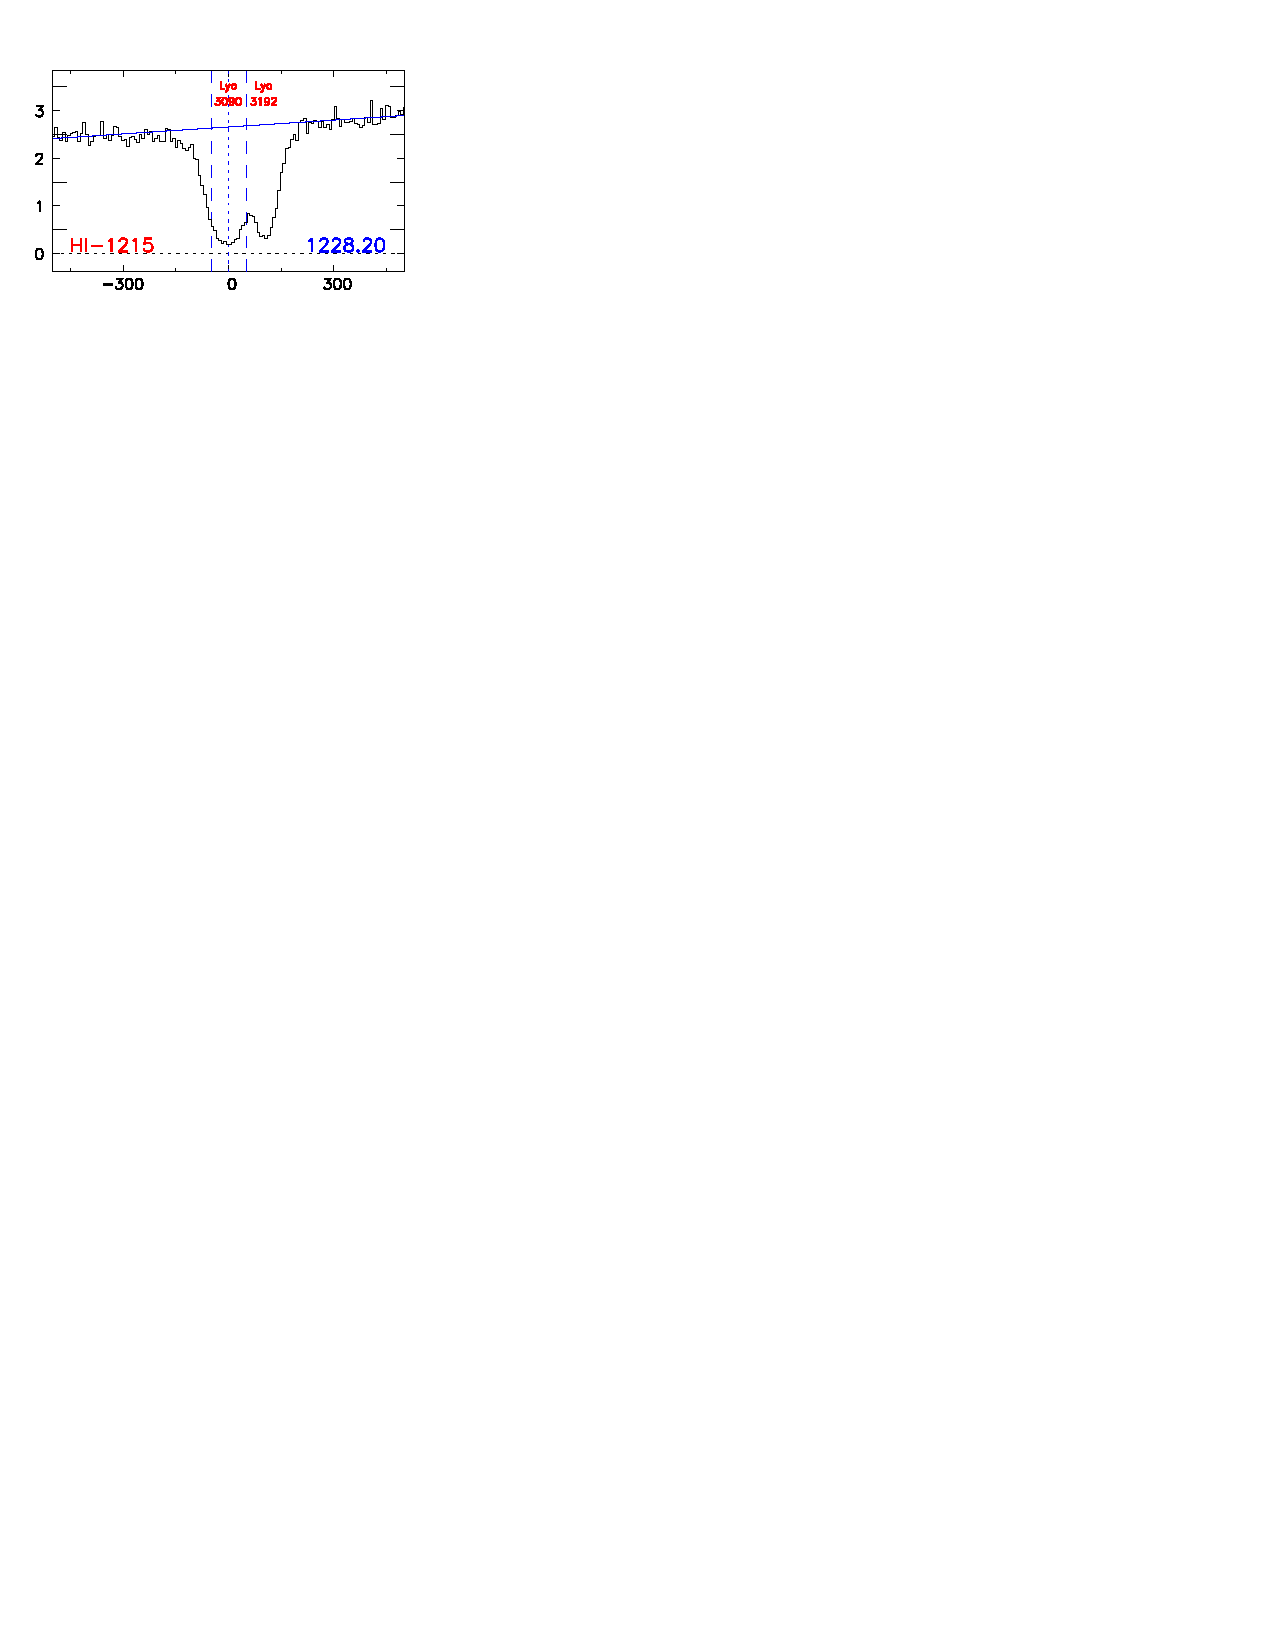
\includegraphics[width=0.87\linewidth]{fig2.pdf}}{\label{line}}
%  \subfigure[]{\includegraphics[width=1.\linewidth]{fig3.pdf}\label{impactmap}}
%  \caption{\small{a) An example of 2 Ly$\alpha$ lines found in the Mrk290 sightline at 3090 and 3192 . b) A map of \textit{all} galaxies within a 500 kpc impact parameter of target Mrk290 sightline and with velocity ($cz$) within 400 $\rm km\, s^{-1}$ of absorption detected at 3192 $\rm km\, s^{-1}$ (central black star). The galaxy NGC5987 ($v=3010$ $\rm km\, s^{-1}$, inclination = $65^{\circ}$) can be unambiguously paired with the Ly$\alpha$ absorption features at $v=3090, 3192$ $\rm km\, s^{-1}$ because it is the largest and closest galaxy in both physical and velocity space to the absorption feature.}}
%\vspace{5pt}
%\end{figure}


To facilitate this decision, we calculate the likelihood, $\mathcal{L}$, of every possible galaxy-absorber pairing as follows:

\begin{equation}
	\mathcal{L} = A e^{-(\frac{\rho}{R_{eff}})^2} e^{-(\frac{\Delta v}{200})^2}.
\end{equation}

\noindent Here $\rho$ is the physical impact parameter, $\Delta v$ the velocity difference between the absorber and the galaxy ($\Delta v = v_{galaxy} - v_{absorber}$), and $A$ is a factor included to increase the likelihood in the case that $\rho \leq R_{eff}$ (in which case $A = 2$, otherwise $A = 1$). 



\section{SUMMARY}



\begin{table}[ht]\footnotesize
\begin{center}
\begin{tabular}{l l l}
 \hline \hline
 Statistic                				&  Blueshifted Absorbers   &     Redshifted Absorbers     \\ 
  \hline \hline
 Number 	          			 		&     	22				&	26			\\
 Mean $EW$    \scriptsize $\rm [m\AA]$    &	$329 \pm 52$ 		&	$245 \pm 34$  	\\
  
\hline
\end{tabular}
\end{center}
  \caption{\small{Average properties of the associated galaxy sample split into red and blue-shifted bins based on $\Delta v$.}}
  \label{resultsTable}
\end{table}


\vspace{10pt}

\indent \textbullet \indent First result


\acknowledgements

This research has made use of the NASA/IPAC Extragalactic Database (NED) which is operated by the Jet Propulsion Laboratory, California Institute of Technology, under contract with the National Aeronautics and Space Administration. Based on observations with the NASA/ESA \textit{Hubble Space Telescope}, obtained at the Space Telescope Science Institute (STScI), which is operated by the Association of Universities for Research in Astronomy, Inc., under NASA contract NAS 5-26555. \textbf{SALT ACKNOWLEDGEMENT}. Spectra were retrieved from the Barbara A. Mikulski Archive for Space Telescopes (MAST) at STScI. Over the course of this study, D.M.F. and B.P.W. were supported by grant AST-1108913, awarded by the US National Science Foundation, and by NASA grants \textit{HST}-AR-12842.01-A, \textit{HST}-AR-13893.01-A, and \textit{HST}-GO-14240 (STScI). 

\facility{HST (COS)}


\nocite{*}
\bibliography{rotation_bib}
\bibliographystyle{apj}

\end{document}
